\section*{Problem  Set 2}

\begin{mdframed}
  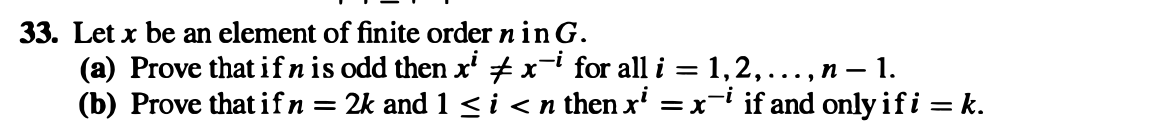
\includegraphics[width=400pt]{img/algebra--nf--2-d8d7.png}
\end{mdframed}

\blue{{\it Note: This exercise was not among those set, but is a sort of lemma for exercise 5.}}

{\it {\bf Intuition:} The only one which is its own inverse is the one ``half way around​'' the cycle, which only exists if $n$ is even. }


\begin{proof}~\\
  {\bf (a)} Suppose there exists $i \in \{1, 2, \ldots, n - 1\}$ such that $x^i = x^{-1}$.
  Then $x^{2i} = e$. Therefore \green{$n | 2i$ and, since $n$ is odd, $n | i$ which
    contradicts $0 < i < n$} (my original argument was more convoluted).

\begin{comment}
  {\bf (b)}\\
  $\implies$~\\
  Suppose $i = k = n/2$. Then $(x^i)^2 = x^{2i} = x^n = e$, therefore $x^i = x^{-i}$.


  $\impliedby$~\\
  Suppose $x^i = x^{-i}$ for some $i \in \{1, 2, \ldots, n - 1\}$. Then
  $(x^i)^2 = x^{2i} = e$. Since $|x| = n$, we have $2i \geq n$. Suppose $2i > n$. Then $2i - n < n$
  since $2i < 2n - 1$. But $x^{2i - n} = x^{2i}x^{-n} = e \cdot e = e$ which is a contradiction
  since $|x| = n$.
\end{comment}
\end{proof}

\begin{mdframed}
In these exercises, $D_{2n}$ has the presentation $D_{2n} = \langle r, s ~|~ r^n = s^2 = 1, rs = sr^\1 \rangle$.
\end{mdframed}

\begin{mdframed}
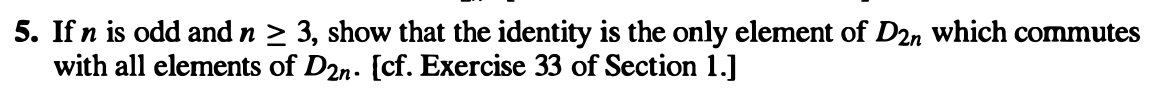
\includegraphics[width=400pt]{img/algebra--nf--2-21ce.png}
\end{mdframed}


\begin{proof}
  Let $n$ be odd and let $x$ be a non-identity element of $D_{2n}$.

  We will exhibit, for any given non-identity element of $D_{2n}$, an element with which it does
  not commute. There are two cases:

  {\bf Case 1}:  $x = r^i$ for some $1 \leq i < n$ \\
  Take $y = s$. Then $xy = r^is$ and $yx = sr^i = r^{-i}s$ via a dihedral relation. But from
  exercise 33a above, for odd $n$, we have $r^i \neq r^{-i}$ for all $1 \leq i < n$, hence $xy \neq yx$.


  {\bf Case 2:}  $x = r^is$ for some $0 \leq i < n$ \\
  Take $y = r$. Then $xy = r^isr = r^ir^\1s = r^{i - 1}s$ and
  \begin{align*}
    xy &= r^isr = r^ir^\1s = r^{i - 1}s
  \end{align*}
  and
  \begin{align*}
    yx &= rr^is = r^{i+1}s.
  \end{align*}
  But $r^{i-1} \neq r^{i+1}$ so $xy \neq yx$.
\end{proof}



\newpage
\begin{mdframed}
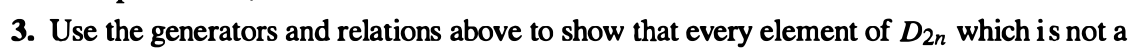
\includegraphics[width=400pt]{img/algebra--nf--2-9bae.png}\\
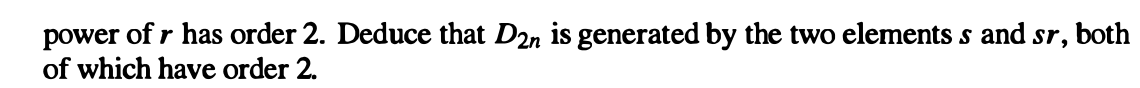
\includegraphics[width=400pt]{img/algebra--nf--2-e89d.png}
\end{mdframed}

\begin{proof}
  First note that every element of $D_{2n}$ which is not a power of $r$ can be written
  as $x = r^is$ for some $0 \leq i < n$, and that such an element is not the identity.

  We see that $x^2 = r^isr^is = sr^{-i}r^is = s^2 = 1$, therefore every element of $D_{2n}$ which is
  not a power of $r$ has order $2$.

  Furthermore note that $s\cdot sr = r$ hence $D_{2n}$ is generated by $s$ and $sr$, since we can
  compute the known generators $s$ and $r$ from them.
\end{proof}


\begin{mdframed}
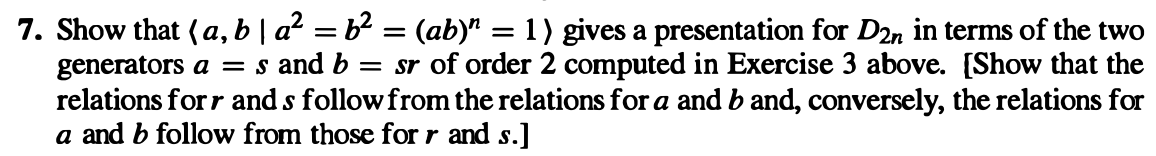
\includegraphics[width=400pt]{img/algebra--nf--2-bb2c.png}
\end{mdframed}


\begin{proof}
  Let $a = s$ and $b = sr$ and note that $ab = s^2r$.

  $\implies$\\
  For the forward implication, suppose $a^2 = b^2 = (ab)^n = 1$. We want to show that the standard
  relations $r^n = s^2 = 1$ and $rs = sr^\1$ hold.

  $s^2 = 1$ is immediate, since we have $a = s$ by definition and $a^2 = 1$ by supposition.

  This gives us $ab = s^2r = 1r = r$. Therefore $r^n = 1$, since $(ab)^n = 1$ by supposition.

  Finally, we have $b = sr$ and $b^2 = 1$, therefore $srsr = 1$. Now, multiplying on the left
  by $s^\1$ and on the right by $r^\1$, we have $rs = s^\1r^\1 = sr^\1$ as required, since
  $s^2 = 1$ implies $s^\1 = s$.



  $\impliedby$\\
  For the reverse implication, suppose $r^n = s^2 = 1$ and $rs = sr^\1$. We want to show that $a^2 = b^2 = (ab)^n = 1$.

  $a^2 = 1$ is immediate since we have $a = s$ by definition and $s^2 = 1$ by supposition.

  Next, we have $ab = s^2r = r$ since $s^2 = 1$ by supposition. Therefore $(ab)^n = 1$ since
  $r^n = 1$ by supposition.

  Finally, we have $rs = sr^\1$ by supposition. Multiplying on the left by $s$ and on the right
  by $r$, gives $srsr = s^2r^\1r$, hence $b^2 = 1$ since $b = sr$ by definition and $s^2 = 1$ by
  supposition.


  We've shown that the relations for $r$ and $s$ in the standard presentation for $D_{2n}$ hold if
  and only if the relations $a^2 = b^2 = (ab)^n = 1$ hold. Therefore the latter relations also give a
  presentation for $D_{2n}$.
\end{proof}




\newpage
\begin{mdframed}
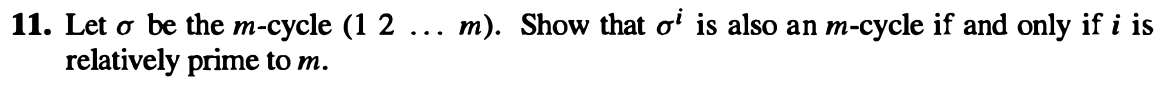
\includegraphics[width=400pt]{img/algebra--nf--2-0db6.png}
\end{mdframed}


\begin{example*}
\begin{verbatim}

sigma^0       1  2  3  4  5  6         (1)(2)(3)(4)(5)(6)
sigma^1       6  1  2  3  4  5         (1  2  3  4  5  6)
sigma^2       5  6  1  2  3  4         (1  3  5)(2  4  6)
sigma^3       4  5  6  1  2  3         (1  4)(2  5)(3  6)
sigma^4       3  4  5  6  1  2         (1  5  3)(2  6  4)
sigma^5       2  3  4  5  6  1         (1  6  5  4  3  2)
sigma^6       1  2  3  4  5  6         (1)(2)(3)(4)(5)(6)
\end{verbatim}
\end{example*}

\begin{proof}
  Under repeated application of $\sigma^i$, the positions visited by the element $1$ form the
  sequence $(ki + 1 \mod m)$ for $k=0, 1, 2, \ldots$.

  Note that an element of this sequence is equal to $1$ if and only if $ki$ is a multiple of $m$.
  Therefore, the first time the sequence returns to $1$ occurs when $ki = \lcm(i, m)$ and we see
  that in the cycle decomposition of $\sigma^i$, the element $1$ belongs to a cycle of
  length $\lcm(i, m) / i$.

  Therefore $\sigma^i$ is an $m$-cycle if and only if $\lcm(i, m) = im$, which is true if and only
  if $i$ and $m$ are relatively prime.

  (To see the last claim, note that from a fundamental theorem regarding $\lcm$ and $\gcd$ we
  have $\lcm(a, b) = ab / \gcd(a, b)$. Therefore $\lcm(i, m) = im$ is true if and only
  if $\gcd(i, m) = 1$, i.e. they are relatively prime.)
\end{proof}



~\\~\\
\begin{mdframed}
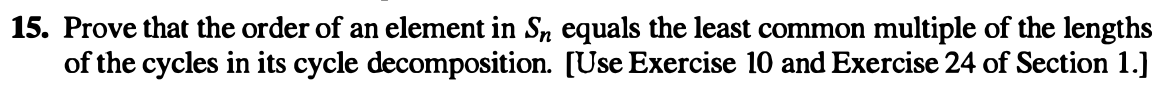
\includegraphics[width=400pt]{img/algebra--nf--2-3beb.png}
\end{mdframed}

\begin{proof}
  Let $x \in S_n$ with cycle decomposition $x = \sigma_1\sigma_2\cdots\sigma_k$ and
  let $N = \lcm(|\sigma_1|, |\sigma_2|, \ldots, |\sigma_k|)$. We must show that $N$ is the smallest positive integer
  such that $x^N = 1$.

  Since the cycles in the decomposition commute and since $N$ is a multiple of the order of every
  cycle in the decomposition, we have $x^N = (\sigma_1\sigma_2\cdots\sigma_k)^N = \sigma_1^N\sigma_2^N\cdots\sigma_k^N = 1^N1^N\cdots1^N = 1$.

  Finally, suppose that $x^M = 1$ for some $M < N$, so that we have
  $\sigma_1^M\sigma_2^M\cdots\sigma_k^M = 1$. But since the cycles in the decomposition are disjoint, this implies (*)
  that $\sigma_i^M = 1$ for every $i = 1, 2, \ldots, k$. Therefore $M$ is a multiple of
  $|\sigma_i|$. But this contradicts the fact that $N$ is the $\lcm$, therefore no such $M < N$ exists.

  To see the claim (*), suppose that $\sigma_i^M \neq 1$ for some $i$. Then, rearranging the order of the
  commuting cycles if necessary, we have $\prod_{j \neq i}\sigma_j^M = (\sigma_i^M)^\1$. But this is impossible: the
  cycles $\sigma_j$ are disjoint, therefore their powers $\sigma_j^M$ are disjoint also, and we cannot form
  the inverse of a non-identity element $\sigma_i^M$ from a product of elements that are disjoint
  with $\sigma_i^M$.
\end{proof}

you can pick any element that is not taken to itself by $\sigma_i^M$ (which must exist because
$\sigma_i^M$ isn't the identity) and then argue that since the $\sigma_j^M$'s are disjoint, this element is
also not taken to itself by their product.



~\\~\\
\begin{mdframed}
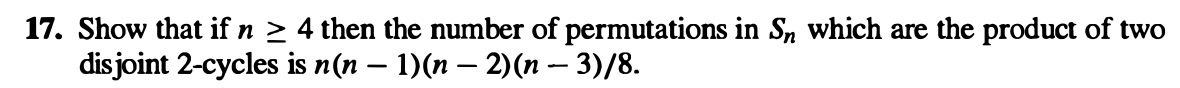
\includegraphics[width=400pt]{img/algebra--nf--2-b38d.png}
\end{mdframed}

\begin{proof}
  For $n \geq 4$, a permutation in $S_n$ which is the product of two disjoint $2$-cycles is defined by
  an unordered specification of two disjoint subsets of $\{1, 2, \ldots, n\}$ of size $2$. The number of
  ways to do so is equal to
  \begin{align*}
    \frac{1}{2}{n \choose 2}{n - 2 \choose 2} = \frac{1}{2}\frac{n(n-1)}{2}\frac{(n-2)(n-3)}{2} = \frac{n(n-1)(n-2)(n-3)}{8},
  \end{align*}
  where the factor of $\frac{1}{2}$ is the double-counting correction that converts a count of
  ordered pairs to a count of unordered pairs.
\end{proof}




~\\~\\
6\\
\begin{mdframed}
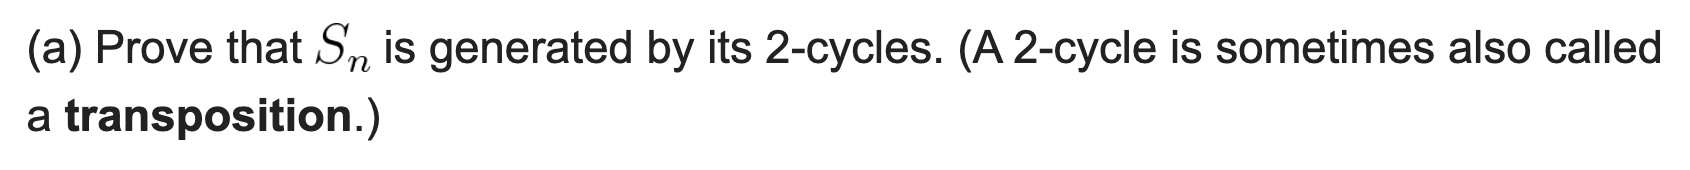
\includegraphics[width=400pt]{img/algebra--nf--2-9aa2.png}
\end{mdframed}

Note: in this proof, $(\cdots)$ is used to denote a permutation in ``one-line​'' notation; not cycle notation.


\begin{proof}
  Let $\sigma \in S_n$ and for $i, j = 1, 2, \ldots, n$, let $\tau_{i,j}$ be the transposition of elements
  $i$ and $j$, where $\tau_{i,i} = e$. We construct $\sigma$ as a product of transpositions as follows:

  \begin{enumerate}
  \item Set $x = (1, 2, \ldots, n)$
  \item For $i = 1, 2, \ldots, n$
    \begin{enumerate}
    \item Let $j$ be the index position of $\sigma(i)$ in $x$.
    \item Apply the transposition $\tau_{i,j}$ to $x$.
    \end{enumerate}
  \end{enumerate}
  Note that:
  \begin{itemize}
  \item Instruction 2a is well-defined because $\sigma(i)$ always occurs at exactly one location in
    $x$. This is true because $\sigma(i) \in \{1, 2, \ldots, n\}$, and $x$ is initialized to a permutation
    of $\{1, 2, \ldots, n\}$, and thereafter is altered only by applying transpositions.
  \item On execution of instruction 2b, $x_i = \sigma(i)$. Thereafter, the value of $x_i$ never changes,
    since in the subsequent iterations of the loop, instruction 2a always sets $j$ equal to the
    index position of $\sigma(i')$ for some $i' > i$.
  \end{itemize}

  Therefore, when this procedure terminates, $x = (\sigma(1), \sigma(2), \ldots, \sigma(n))$, i.e.
  $x$ is $\sigma$ written in ``one-line​'' notation. Since we used only transpositions in the algorithm,
  and $\sigma$ was arbitrary, $S_n$ is generated by its transpositions.
\end{proof}

Alternative proof:

\begin{proof}
  Note that any cycle can be written as a product of transpositions:
  \begin{align*}
     (a_1, a_2, \ldots, a_k) = (a_1, a_k)(a_1, a_{k-1}) \cdots (a_1, a_2).
  \end{align*}
  Therefore any $\sigma \in S_n$ can be written as a product of transpositions by first forming its cycle
  decomposition and then replacing each cycle in the decomposition with a product of transpositions
  formed as above.
\end{proof}


\begin{mdframed}
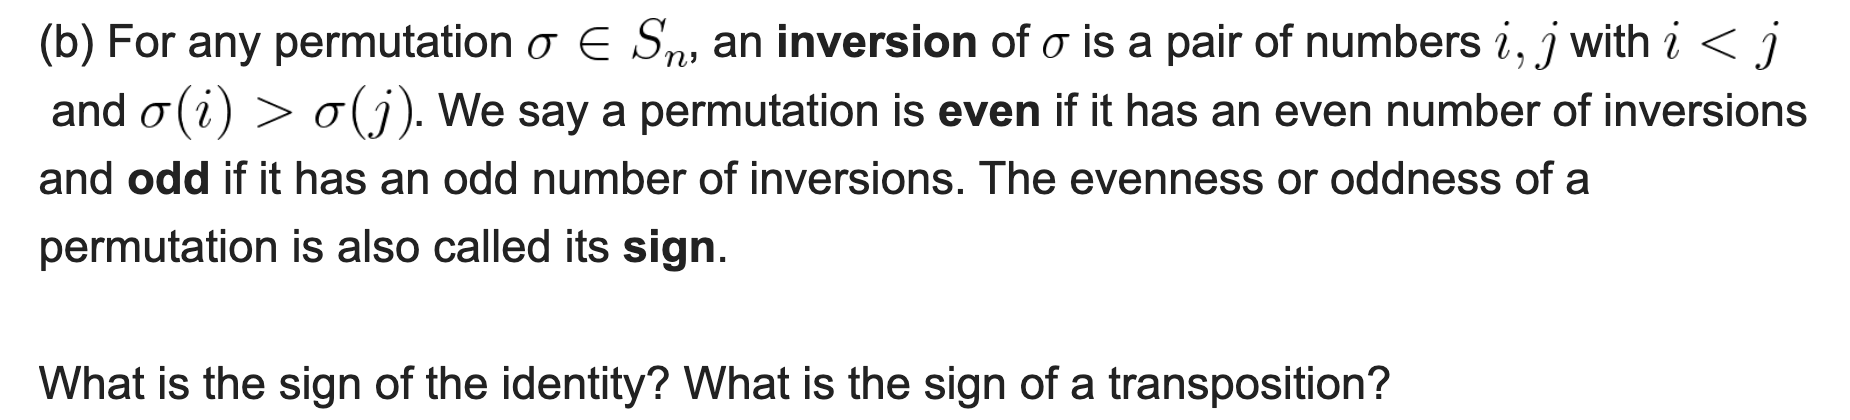
\includegraphics[width=400pt]{img/algebra--nf--2-d8ce.png}
\end{mdframed}


The identity is even since it has zero inversions.

A transposition is odd. To see this, consider the transposition $(i, j)$. Clearly it has
the $\{i, j\}$ inversion. And we also get $2(|i - j| - 1)$ additional inversions since, for every
inversion induced by $i$ "crossing over" an intervening position, there is a matching inversion
induced by $j$ "crossing over" in the opposite direction. So the total number is odd.

For example, the transposition $(1, 4)$ has $5$ inversions:
\begin{mdframed}
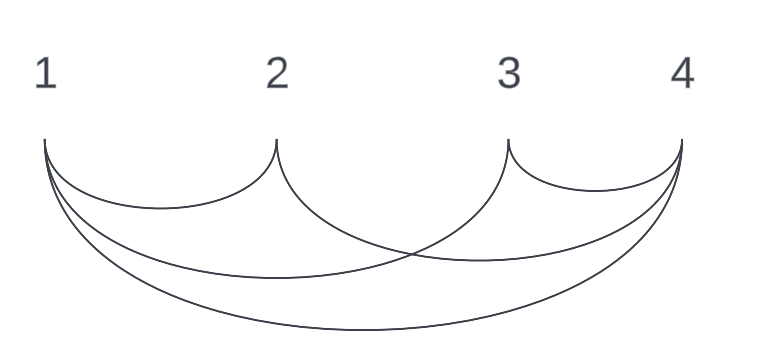
\includegraphics[width=400pt]{img/abstract-algebra--nf--2-e92f.png}
\end{mdframed}




\begin{mdframed}
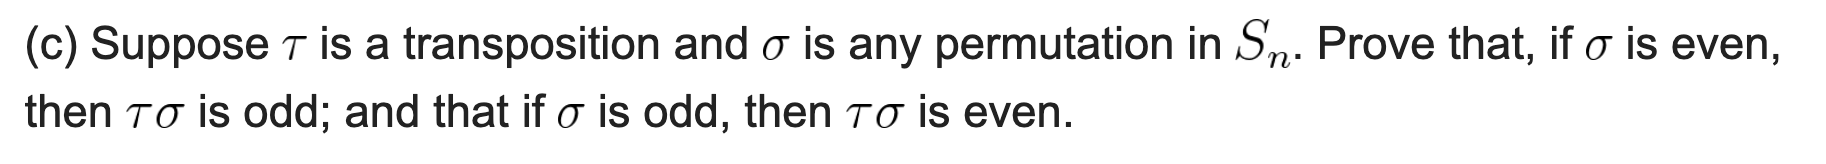
\includegraphics[width=400pt]{img/algebra--nf--2-179c.png}
\end{mdframed}

\begin{mdframed}
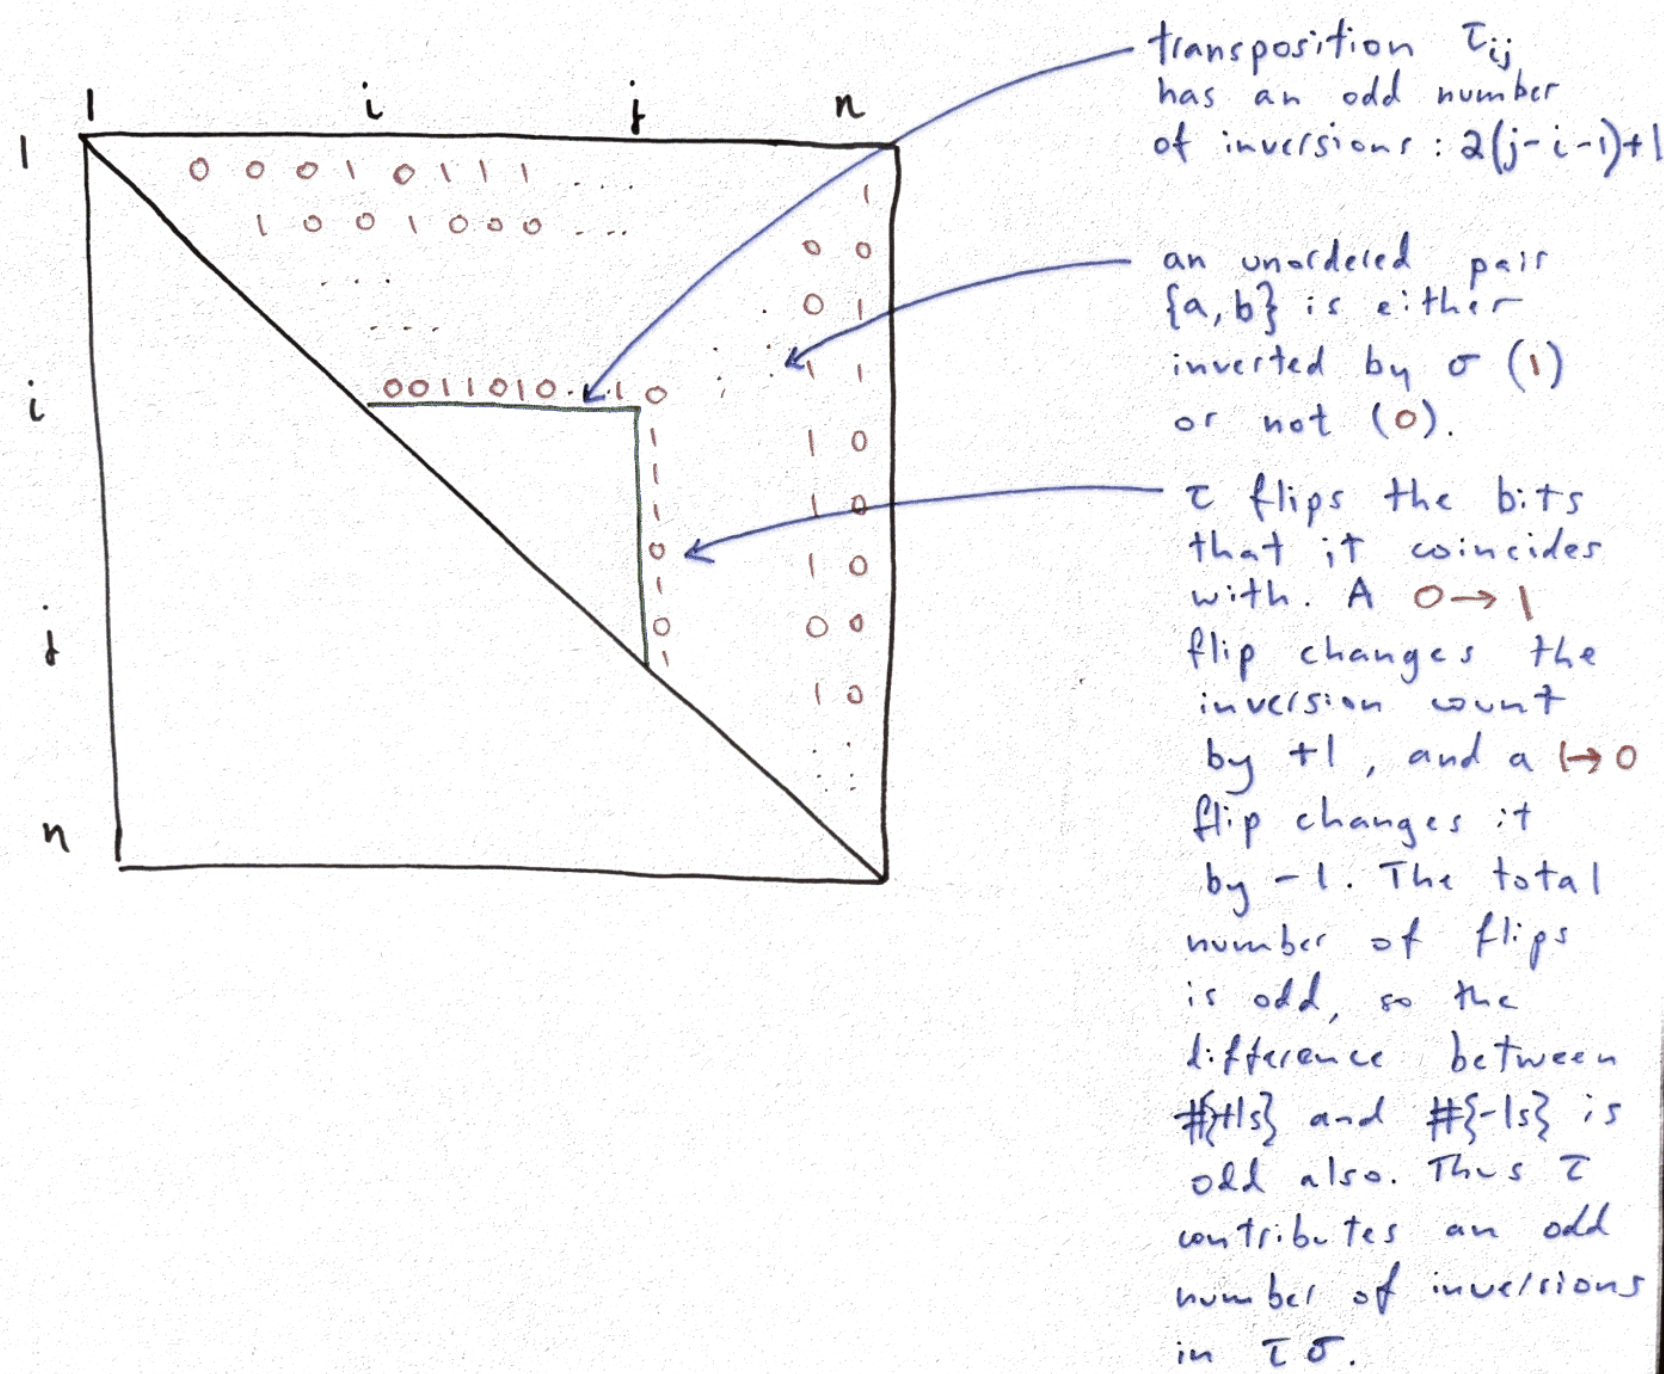
\includegraphics[width=400pt]{img/abstract-algebra--nf--2-4dc0.png}
\end{mdframed}


\begin{proof}
  Let $\sigma \in S_n$ be any permutation, let $\tau \in S_n$ be the transposition of $i$ and $j$, and for
  any $\rho \in S_n$ define
  \begin{align*}
    \delta^{(\rho)}_{a,b} =
    \begin{cases}
      1 &~~~\text{if}~\{a, b\}~\text{is an inversion of}~\rho\\
      0 &~~~\text{otherwise},
    \end{cases}
  \end{align*}
  and
  \begin{align*}
    I^-(\rho) &=  \sum_{\substack{l > k\\k, l \in \{1, 2, \ldots, n\} - \{i, j\}}}\delta^{(\rho)}_{kl}\\
    I^+(\rho) &=  \sum_{\substack{l > k\\k \in \{i, j\} ~\text{or}~ l \in \{i, j\}}}\delta^{(\rho)}_{kl},
  \end{align*}
  where indices $k$ and $l$ range over $1, 2, \ldots, n$. Thus $I(\rho) = I^-(\rho) + I^+(\rho)$ is the number of
  inversions of $\rho$. Assume WLOG that $j > i$ and note that the summation in the definition
  of $I^+(\rho)$ ranges over an odd number $2(j - i -1) + 1$ of elements.

  Next, note that every inversion of $\tau$ involves either $i$ or $j$. Therefore
  \begin{align*}
    \delta^{(\tau\sigma)}_{kl} =
    \begin{cases}
      \delta^{(\sigma)}_{kl} &~~~k, l \in \{1, 2, \ldots, n\} - \{i, j\}\\
      1 - \delta^{(\sigma)}_{kl} &~~~\text{either}~k \in \{i, j\} ~\text{or}~ l \in \{i, j\},
    \end{cases}
  \end{align*}

  hence $I^-(\tau\sigma) = I^-(\sigma)$ and
  \begin{align*}
    I^+(\tau\sigma) &= 2(j - i -1) + 1 -  \sum_{\substack{l > k\\k \in \{i, j\} ~\text{or}~ l \in \{i, j\}}}\delta^{(\sigma)}_{kl}.
  \end{align*}





  First note that an inversion

  First note that every inversion of $\tau$ involves either $i$ or $j$. Therefore if
  neither $\sigma(k)$ nor $\sigma(l)$ is $i$ or $j$ then $\{k, l\}$ is an inversion of
  $\tau_{i,j}\sigma$ if and only if it is an inversion of $\sigma$.

  So what we need to do is count
  \begin{align*}
    \Big\{\{k, l\} ~\big |~ \{k, l\} \text{~is an inversion of~} \tau_{i,j}\sigma \text{~and~} k \in \{i, j\} \text{~or~} l \in \{i, j\}\Big\}.
  \end{align*}


  If $\sigma = 1$ then the claim is true since $|1| = 0$ is even and $|\tau\sigma| = |\tau|$ which we've already
  proved is odd.

  [incomplete and informal hereafter]\\

  Recall the argument for $\tau_{i,j}$ being odd above: it involved the $\{i, j\}$ inversion
  and $2|i - j|$ inversions involving $i$ or $j$ and one of the positions between $i$ and $j$.

  Assume WLOG that $i < j$.

  First note that if $\sigma$ does not touch any position in $i, i+1, \ldots, j$ then $\sigma$ and
  $\tau$ do not interact and the claim is true: $\sigma$ does whatever it does, and $\tau$ adds its odd number
  of inversions.

  What remains is to prove the claim for any $\sigma$ that touches at least one position in the region
  labeled $C$ here:

    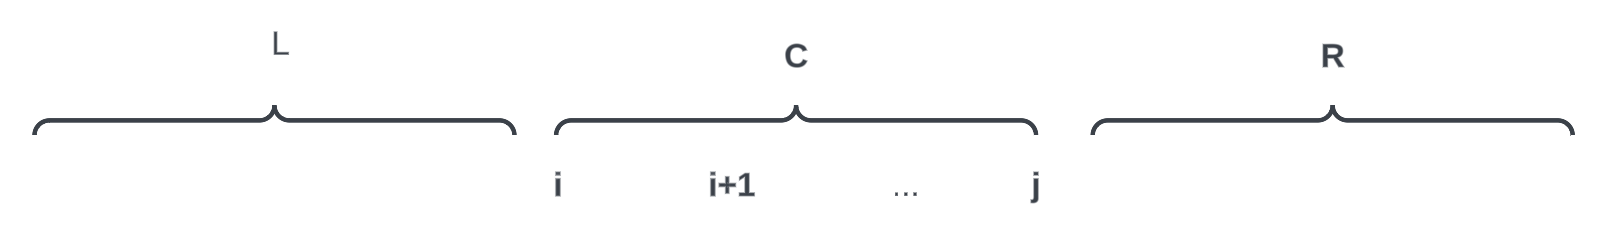
\includegraphics[width=400pt]{img/abstract-algebra--nf--2-b9b0.png}








  Next, let's consider the simplest possible case that we haven't covered: $\sigma$ is a $2$-cycle that



\end{proof}


\begin{mdframed}
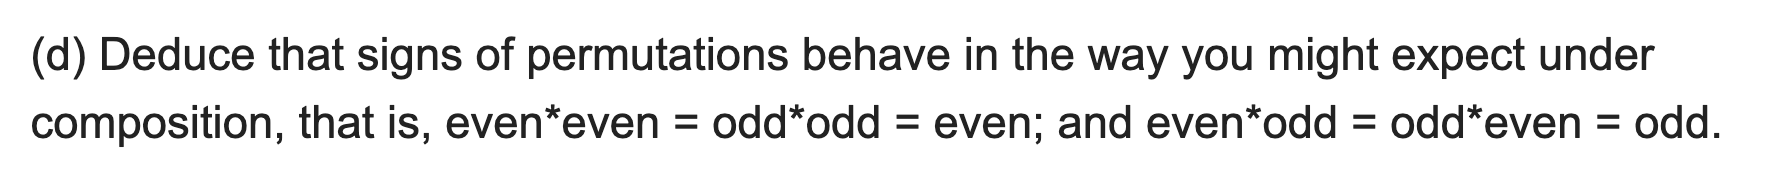
\includegraphics[width=400pt]{img/algebra--nf--2-05a9.png}
\end{mdframed}

\begin{proof}
  First note that it follows from result (c) above that the product of an even number of
  transpositions is an even permutation, and the product of an odd number of transpositions is an
  odd permutation. To see this, note that we can rewrite any product $\tau_1\tau_2\cdots\tau_K$
  as $\tau_1(\tau_2(\cdots(\tau_K(1))))$ and, since $1$ is an even permutation, it follows from
  result (c) that this product is even if and only if $K$ is even.

  Therefore, since $S_n$ is generated by its transpositions, an even permutation can be written as
  a product of an even number of transpositions (but not an odd number) and an odd permutation can
  be written as a product of an odd number of transpositions (but not an even number).

  The desired result follows: if $\sigma_1$ and $\sigma_2$ are both even (resp. odd), then write them both as
  products of even (resp. odd) numbers of transpositions, and observe that the total number of
  transpositions in the product of the two is even, and therefore that that product is an even
  permutation. Alternatively if one of $\sigma_1$ and $\sigma_2$ is odd and the other even, then write one as
  a product of an odd number of transpositions and the other as the product of an even number of
  transpositions, and observe that the total number of transpositions in the product of the two is
  odd, and therefore that that product is an odd permutation.
\end{proof}
